%% ==============================
\chapter{Methods}
\label{sec:methods}
%% ==============================
Questions to ask:
\begin{enumerate}
    \item Describe the research design, data collection, and data analysis methods you will employ to address your research question.
    \item What are the main assumptions and limitations of the methodology?
    \item How is data collected, processed, and analyzed? 
    \item (If relevant) What statistical or computational techniques are used to analyze the data?  
    \item How is the validity and reliability of the methodology ensured? 
\end{enumerate}

The general methodology of this work follows a iterative design principle. First related work with specific approaches were analysed. These approaches used benchmark environments to test their implementation and compare it to previous approaches. These benchmarks were taken as a starting point for development of the planner for this work. In the first evaluation phase a comparison of the developed planner with other algorithms was done on the same benchmarks. A new metric was developed to quantify the disturbance of public space. In the next step, the hierarchical planner was tested with a model of a real building. To combine these concepts, they were integrated in the \gls{nav_2} stack and tested in a simulated hospital environment. Throughout these steps, continuous improvement was done on the code.

One limitation of the method of his work is that no comparative evaluation of the developed hierarchical planner with the related work was conducted. This is due to the fact, that the focus of this work is the implementation on a real robot with ROS 2, while older approaches used different frameworks and did not publish the code online as open-source. Also the optimization of the developed planner in terms of computation speed was not scope of this work. This results in the lack of direct comparisons of planning times and other metrics of the hierarchical planner. A comparison of the straight path planner was done as described in the following sections.

%% ==============================
\section{Existing Benchmarks}
\label{sec:benchmarks}
%% ==============================
 As seen in the literature review in Chapter \ref{sec:state_of_the_art} most related works used common benchmarks to test their approaches. In specific, the benchmark from \cite{ryu_hierarchical_2020} was used for testing the hierarchy creation and two-level hierarchical planning. This environment is a map of a real building. It was originally recorded by Stachniss \cite{cyrill_stachniss_robotics_2015} on the Campus of the University of Freiburg, see Figure \ref{fig:freiburg_benchmark}. The second benchmark environment was previously shown in Figure \ref{fig:htm_global_comparison} and is primarily used to compare the straight path planner against the previous approaches. It was also used by Hou \cite{hou_straight_2021} with the SIRRT* planner as well as by Beeson \cite{beeson_towards_2005} with the EVG planner.

\begin{figure}[h]
    \centering
    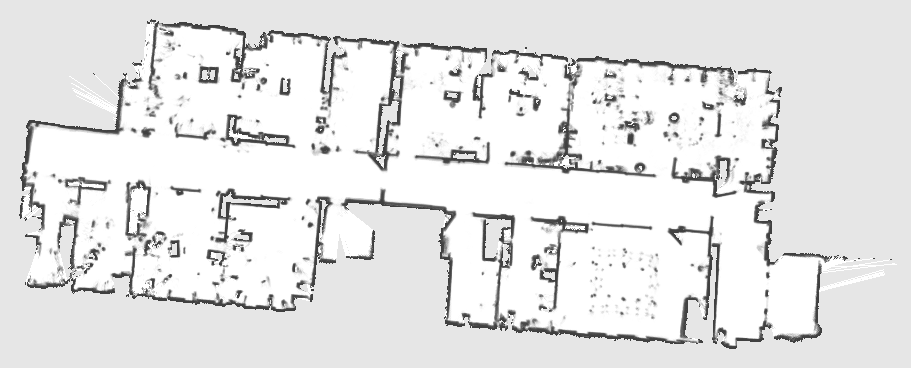
\includegraphics[width=0.75\textwidth]{figures/30_methods/freiburg_benchmark.png}
    \caption[The benchmark environment for hierarchy creation and straight path planning]{The benchmark environment for hierarchy creation and straight path planning recorded in the University of Freiburg (Source: \cite{cyrill_stachniss_robotics_2015})}
    \label{fig:freiburg_benchmark}
\end{figure}

In the first evaluation phase of the iterative process the developed straight path planner is tested on these benchmark environments and compared to the related work and common path planner algorithms. To ensure reliable and statistically significant results each planner is tested on different benchmarks and the corresponding submaps of a single room. Each planner produces a number of paths resulting from the number of combination of start and goal positions. These positions consist of \(n_r\) randomly sampled points in the driveable area and all bridge points \(n_b\) of the environment or submap. The total number of paths \(n_{\text{paths}}\) results from choosing two of these points from the start and goal points and repeating this for all possible combinations. This can be expressed by the formular of the binomial coefficient while \(k\) equals 2 because there is only one starting point and one goal point, see the Equation \ref{equ:binomial_coefficient}.
\begin{equation} \label{equ:binomial_coefficient}
    n_{\text{paths}} = \binom{n_r + n_b}{2} = \frac{(n_r + n_b)!}{2! ((n_r + n_b)-2)!}
\end{equation}
In the case of one example room there are 3 bridge points \(n_b\) and additionally 10 random points \(n_r\), resulting in 78 paths. In the case of the complete floor from the benchmark in Figure \ref{fig:freiburg_benchmark} \(n_b = 27\) and \(n_r = 20\) resulting in 1081 paths. These paths were then evaluated on the following metrics:
\begin{enumerate}
  \item \textbf{Success rate}: Percentage of valid paths found
  \item \textbf{Path length}: Total length from start to goal in pixels
  \item \textbf{Planning time}: Total time for planning including smoothing
  \item \textbf{Path smoothness}: Sum of deviation angles divided by path length
  \item \textbf{Obstacle clearance}: Mean distance from path to obstacles
  \item \textbf{Distance deviation}: Standard deviation of the distance between path and obstacle
  \item \textbf{Distance to centroid}: Mean distance from path to centroid of the room
  \item \textbf{Disturbance of public space}: Largest open area inside roadmap divided by total room area (Details in Chapter \ref{sec:new_metric})
\end{enumerate}

%% ==============================
\section{New Metric for Disturbance of Public Space}
\label{sec:new_metric}
%% ==============================
In the problem statement in chapter \ref{sec:problem_statement} the need for straight, deterministic and human-predictable paths is presented. In specific situations it is important to drive close to the walls and not directly through the room. Such a scenario was presented in Figure \ref{problem_disturbance}. To measure the capability of the planner to produce paths that have a low disturbance of public space by design, a new metric has to be invented. Until now there is no such metric in literature as most path planning problems focus on finding the shortest possible solution. In contrast, this work focuses on straight paths and predictability. To avoid driving directly through a major traffic way for humans or through the queue of an information desk, this planner tries to stay close and parallel to the walls. This new metric provides a method to quantify this behavior. In comparison to most path metrics and all of the metrics mentioned in the previous chapter, this new metric can not be calculated from one single solution path. It gives a value for how well all possible paths in the map combined avoid the disturbance of public space. The process of obtaining this value for one single room is described in the following:

\begin{enumerate}
    \item Get all bridge points \(n_b\) connecting this room to adjacent rooms or other hierarchies
    \item Sample \(n_r\) random points inside the valid area (default \(n_r = 10\))
    \item Plan paths for all possible connections given by the equation \ref{equ:binomial_coefficient}
    \item Overlay all paths on the original room environment \(R\)
    \item Segment the room into connected components \(CC_{\text{free}}\) which are not separated by paths
    \item Get the largest connected components by area \(CC_{\text{free, max}} = \max \{\text{area}(CC_{\text{free}})\}\)
    \item Divide by the total room area and subtract from 1 to get the disturbance value \(D\) as in equation \ref{equ:disturbance}
\end{enumerate}
\begin{equation}
\label{equ:disturbance}
    D = 1 - \frac{\max \{\text{{area}}(CC_{\text{{free}}})\}}{{\text{{area}}(R)}}
\end{equation}

This results in a metric for the disturbance of public space for a single room where a low value is indicating a desirable behavior for a mobile robot. In Figure \ref{fig:disturbance_example} a comparison of the metric on a room from the second benchmark is shown.

\begin{figure}[h]
    \captionsetup[subfigure]{justification=centering}
    \centering
    \begin{subfigure}{.5\textwidth}
      \centering
      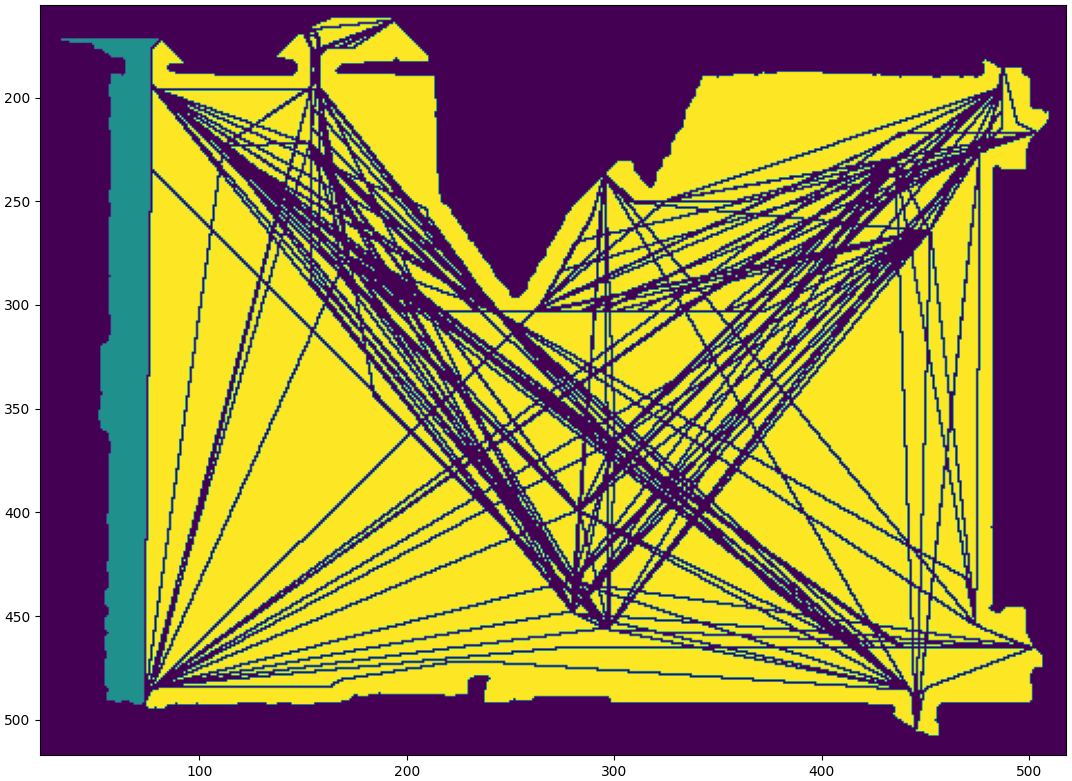
\includegraphics[width=\textwidth]{figures/30_methods/room9_disturbance_astar_smooth.png}
      \caption{Planner: A*, \(D = 0.95\)}
      \label{fig:sub1}
    \end{subfigure}%
    \begin{subfigure}{.5\textwidth}
      \centering
      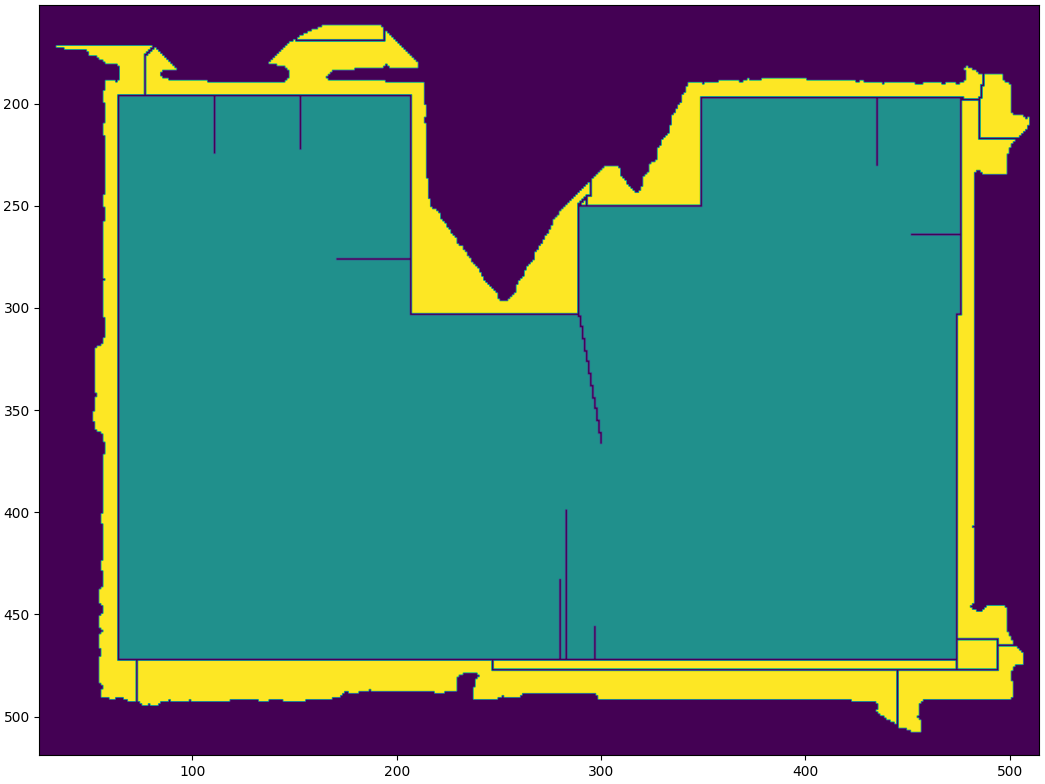
\includegraphics[width=.975\textwidth]{figures/30_methods/room9_disturbance_ilir_smooth.png}
      \caption{Planner: ILIR, \(D = 0.20\)}
      \label{fig:sub2}
    \end{subfigure}
    \caption[Example of the metric for disturbance of public space]{Example of the metric for disturbance of public space with \(n_r=10\), \(n_b=9\), \(n_{\text{paths}}=171\). The area of the original room \(R\) in yellow and turquoise, the paths and the walls in purple and the largest free area \(CC_{\text{free, max}}\) in turquoise.}
    \label{fig:disturbance_example}
\end{figure}

%% ==============================
\section{Simulation}
\label{sec:simulation}
%% ==============================
After developing the hierarchy creation and the two-level hierarchical planning a more complex environment was needed to evaluate the hierarchical planning with arbitrary hierarchical levels and connections between them. For this purpose the campus of our research lab was modeled as graph and used for planning. This environment is complex in means of hierarchical connections, for example some stairs are connecting the second floor diagonal to the terrace of the first floor, which is itself shaped in a ring connecting to all other buildings. This makes this environment more complex than a simple building with one vertical connection through an elevator as used by previous work, like \cite{gregoric_autonomous_2022} or \cite{cagigas_hierarchical_2005}. A rendering of the campus and the corresponding graph can bee seen in Figure \ref{}

\todo{insert two sided picture of LTC real and LTC graph}

Both concept, the hierarchical planner and the straight path planner were combined and integrated into the \gls{nav_2} stack for \gls{ros_2}. For fast testing this was done in an simulated hospital environment. This helps in debugging and accelerates the developement. The publicly available "AWS RoboMaker Hospital World" from Amazon \cite{aws_robotics_aws_2023} was used. In Figure \ref{fig:aws_hospital} the simulated hospital is shown. The advantage of this environment is that it also provides models for two and three floors. From this simulation the gap to the real world is small and it was finally implemented on the real PeTRA robot.

\begin{figure}[h]
    \centering
    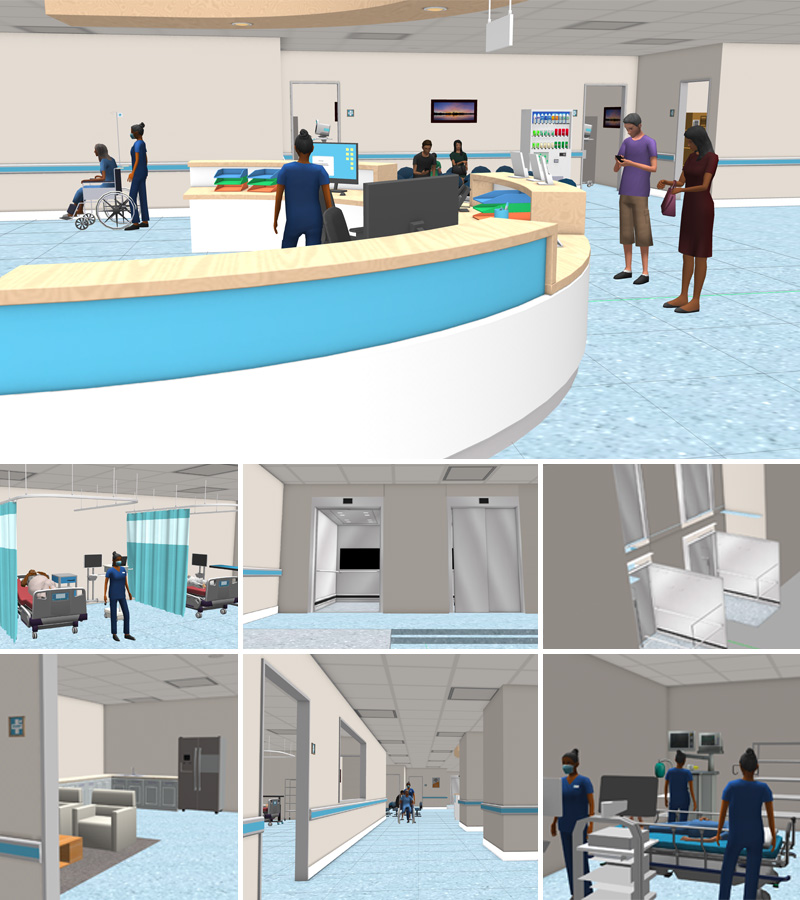
\includegraphics[width=0.5\textwidth]{figures/30_methods/hospital_world.jpg}
    \caption[The "AWS RoboMaker Hospital World" simulation environment for Gazebo]{The "AWS RoboMaker Hospital World" simulation environment for Gazebo. (Source: \cite{aws_robotics_aws_2023})}
    \label{fig:aws_hospital}
\end{figure}